\documentclass[12pt]{beamer}
\usepackage{../Estilos/BeamerFC}
\usepackage{../Estilos/ColoresLatex}
\usepackage{courier}
\usepackage{listingsutf8}
\usepackage{listings}
\usepackage{xcolor}
\usepackage{textcomp}
\usepackage{color}
\definecolor{deepblue}{rgb}{0,0,0.5}
\definecolor{brown}{rgb}{0.59, 0.29, 0.0}
\definecolor{OliveGreen}{rgb}{0,0.25,0}
% \usepackage{minted}

\DeclareCaptionFont{white}{\color{white}}
\DeclareCaptionFormat{listing}{\colorbox{gray}{\parbox{0.98\textwidth}{#1#2#3}}}
\captionsetup[lstlisting]{format=listing,labelfont=white,textfont=white}
\renewcommand{\lstlistingname}{Código}


\definecolor{Code}{rgb}{0,0,0}
\definecolor{Keywords}{rgb}{255,0,0}
\definecolor{Strings}{rgb}{255,0,255}
\definecolor{Comments}{rgb}{0,0,255}
\definecolor{Numbers}{rgb}{255,128,0}

\makeatletter

\newif\iffirstchar\firstchartrue
\newif\ifstartedbyadigit
\newif\ifprecededbyequalsign

\newcommand\processletter
{%
  \ifnum\lst@mode=\lst@Pmode%
    \iffirstchar%
        \global\startedbyadigitfalse%
      \fi
      \global\firstcharfalse%
    \fi
}

\newcommand\processdigit
{%
  \ifnum\lst@mode=\lst@Pmode%
      \iffirstchar%
        \global\startedbyadigittrue%
      \fi
      \global\firstcharfalse%
  \fi
}

\lst@AddToHook{OutputOther}%
{%
  \lst@IfLastOtherOneOf{=}
    {\global\precededbyequalsigntrue}
    {}%
}

\lst@AddToHook{Output}%
{%
  \ifprecededbyequalsign%
      \ifstartedbyadigit%
        \def\lst@thestyle{\color{orange}}%
      \fi
    \fi
  \global\firstchartrue%
  \global\startedbyadigitfalse%
  \global\precededbyequalsignfalse%
}

\lstset{ 
language=Python,                % choose the language of the code
basicstyle=\footnotesize\ttfamily,       % the size of the fonts that are used for the code
numbers=left,                   % where to put the line-numbers
numberstyle=\scriptsize,      % the size of the fonts that are used for the line-numbers
stepnumber=1,                   % the step between two line-numbers. If it is 1 each line will be numbered
numbersep=5pt,                  % how far the line-numbers are from the code
backgroundcolor=\color{white},  % choose the background color. You must add \usepackage{color}
showspaces=false,               % show spaces adding particular underscores
showstringspaces=false,         % underline spaces within strings
showtabs=false,                 % show tabs within strings adding particular underscores
frame=single,   		% adds a frame around the code
tabsize=2,  		% sets default tabsize to 2 spaces
captionpos=t,   		% sets the caption-position to bottom
breaklines=true,    	% sets automatic line breaking
breakatwhitespace=false,    % sets if automatic breaks should only happen at whitespace
escapeinside={| |},  % if you want to add a comment within your code
stringstyle =\color{OliveGreen},
otherkeywords={as, np.array, np.concatenate, np.linspace, linspace, interpolate.interp1d, kind, plt.plot, .copy, np.arange, np.cos, np.pi, lw, ls, label, splrep, splev, plt.legend, loc, plt.title, plt.ylim, plt.show, sign, math.ceil, math.log, np.sqrt, np.exp, np.zeros, plt.xlabel, plt.ylabel, plt.xlim, np.identity, random, np.dot, np.outer, np.diagonal },             % Add keywords here
keywordstyle = \color{blue},
commentstyle = \color{darkcerulean},
identifierstyle = \color{black},
literate=%
         {á}{{\'a}}1
         {é}{{\'e}}1
         {í}{{\'i}}1
         {ó}{{\'o}}1
         {ú}{{\'u}}1
%
%keywordstyle=\ttb\color{deepblue}
%fancyvrb = true,
}

\lstdefinestyle{FormattedNumber}{%
    literate={0}{{\textcolor{red}{0}}}{1}%
             {1}{{\textcolor{red}{1}}}{1}%
             {2}{{\textcolor{red}{2}}}{1}%
             {3}{{\textcolor{red}{3}}}{1}%
             {4}{{\textcolor{red}{4}}}{1}%
             {5}{{\textcolor{red}{5}}}{1}%
             {6}{{\textcolor{red}{6}}}{1}%
             {7}{{\textcolor{red}{7}}}{1}%
             {8}{{\textcolor{red}{8}}}{1}%
             {9}{{\textcolor{red}{9}}}{1}%
             {.0}{{\textcolor{red}{.0}}}{2}% Following is to ensure that only periods
             {.1}{{\textcolor{red}{.1}}}{2}% followed by a digit are changed.
             {.2}{{\textcolor{red}{.2}}}{2}%
             {.3}{{\textcolor{red}{.3}}}{2}%
             {.4}{{\textcolor{red}{.4}}}{2}%
             {.5}{{\textcolor{red}{.5}}}{2}%
             {.6}{{\textcolor{red}{.6}}}{2}%
             {.7}{{\textcolor{red}{.7}}}{2}%
             {.8}{{\textcolor{red}{.8}}}{2}%
             {.9}{{\textcolor{red}{.9}}}{2}%
             {\ }{{ }}{1}% handle the space
         ,%
          %mathescape=true
          escapeinside={__}
          }



\usetheme{Warsaw}
\usecolortheme{seahorse}
%\useoutertheme{default}
\setbeamercovered{invisible}
% or whatever (possibly just delete it)
\setbeamertemplate{section in toc}[sections numbered]
\setbeamertemplate{subsection in toc}[subsections numbered]
\setbeamertemplate{subsection in toc}{\leavevmode\leftskip=3.2em\rlap{\hskip-2em\inserttocsectionnumber.\inserttocsubsectionnumber}\inserttocsubsection\par}
\setbeamercolor{section in toc}{fg=blue}
\setbeamercolor{subsection in toc}{fg=blue}
\setbeamercolor{frametitle}{fg=blue}
\setbeamertemplate{caption}[numbered]

\setbeamertemplate{footline}
\beamertemplatenavigationsymbolsempty
\setbeamertemplate{headline}{}


\makeatletter
\setbeamercolor{section in foot}{bg=gray!30, fg=black!90!orange}
\setbeamercolor{subsection in foot}{bg=blue!30}
\setbeamercolor{date in foot}{bg=black}
\setbeamertemplate{footline}
{
  \leavevmode%
  \hbox{%
  \begin{beamercolorbox}[wd=.333333\paperwidth,ht=2.25ex,dp=1ex,center]{section in foot}%
    \usebeamerfont{section in foot} \insertsection
  \end{beamercolorbox}%
  \begin{beamercolorbox}[wd=.333333\paperwidth,ht=2.25ex,dp=1ex,center]{subsection in foot}%
    \usebeamerfont{subsection in foot}  \insertsubsection
  \end{beamercolorbox}%
  \begin{beamercolorbox}[wd=.333333\paperwidth,ht=2.25ex,dp=1ex,right]{date in head/foot}%
    \usebeamerfont{date in head/foot} \insertshortdate{} \hspace*{2em}
    \insertframenumber{} / \inserttotalframenumber \hspace*{2ex} 
  \end{beamercolorbox}}%
  \vskip0pt%
}
\makeatother

\makeatletter
\patchcmd{\beamer@sectionintoc}{\vskip1.5em}{\vskip0.8em}{}{}
\makeatother

%\newlength{\depthofsumsign}
%\setlength{\depthofsumsign}{\depthof{$\sum$}}
% \newcommand{\nsum}[1][1.4]{% only for \displaystyle
%     \mathop{%
%         \raisebox
%             {-#1\depthofsumsign+1\depthofsumsign}
%             {\scalebox
%                 {#1}
%                 {$\displaystyle\sum$}%
%             }
%     }
% }
\def\scaleint#1{\vcenter{\hbox{\scaleto[3ex]{\displaystyle\int}{#1}}}}
\def\scaleoint#1{\vcenter{\hbox{\scaleto[3ex]{\displaystyle\oint}{#1}}}}
\def\bs{\mkern-12mu}

\usefonttheme{serif}

\title{\large{Tema 1 - Errores y artimética de punto flotante}}
\author{M. en C. Gustavo Contreras Mayén}
\date{ }

\begin{document}
\maketitle

\section*{Contenido}
\frame[allowframebreaks]{\frametitle{Contenido} \tableofcontents[currentsection, hideallsubsections]}

\section{Números en la computadora}
\frame{\tableofcontents[currentsection, hideothersubsections]}
\subsection{Los números en la computadora}

\begin{frame}
\frametitle{Los números en la computadora}
Las computadoras son herramientas muy poderosas, pero tienen un alcance finito.
\\
\bigskip
\pause
Un problema que se presenta en el diseño de computadora es cómo representar un número arbitrario usando una cantidad finita de espacio de memoria y cómo tratar con las limitaciones que surgen de esta representación.
\end{frame}
\begin{frame}
\frametitle{Los números en la computadora}
Como consecuencia de que las memorias de la computadora se basan en un estado de magnetización o electrónico de un giro que apunta hacia arriba o hacia abajo, las unidades más elementales de memoria de la computadora son los dos enteros binarios (bits) $0$ y $1$.
\end{frame}
\begin{frame}
\frametitle{Los números en la computadora}
Esto significa que la forma en que se almacenan los números en memoria, es como cadenas largas de ceros y unos, es decir, de modo binario.
\end{frame}

\subsection{Rango de operación}

\begin{frame}
\frametitle{Rango de representación}
De esta manera: $N$ bits almacena números enteros en el rango $[0, 2^{N}]$, pero debido a que el signo del número entero está representado por el primer bit (un bit cero para números positivos), el rango real disminuye a:
\pause
\begin{align*}
\big[ 0, 2^{N- 1} \big]
\end{align*}
\end{frame}
\begin{frame}
\frametitle{Otras bases de operación}
La representación binaria de números a través de ceros y unos, funciona y opera bien para las computadoras, pero no para los usuarios.
\\
\bigskip
\pause
Es por ello que las cadenas binarias se convierten en números octal, decimal o hexadecimal antes de que los resultados se presenten a los usuarios.
\end{frame}
\begin{frame}
\frametitle{Otras bases de operación}
Los números octales y hexadecimales son también oportunos porque en la conversión no se pierde precisión.
\\
\bigskip
\pause
Pero no todo queda bien ya que nuestras reglas decimales de aritmética no funcionan para ellos.
\end{frame}

\subsection{Aritmética binaria}

\begin{frame}
\frametitle{Desventaja de la aritmética binaria}
La conversión a números decimales hace que los números sean más fáciles de trabajar, pero a menos que el número sea una potencia de $2$, el proceso conduce a una disminución en la precisión.
\end{frame}
\begin{frame}
\frametitle{Longitud de palabra}
Una descripción de un sistema informático particular indica normalmente la \emph{longitud de la palabra}, siendo el número de bits utilizados para almacenar un número.
\\
\bigskip
\pause
La longitud se expresa en bytes, donde:
\pause
\begin{align*}
1 \text{ byte} \equiv 1 \text{ B} \equiv 8 \: \si{\bit}
\end{align*}
\end{frame}

\subsection{Unidades de medida}

\begin{frame}
\frametitle{Unidades de medida}
Tanto la memoria como el almacenamiento se mide en bytes, kilobytes, megabytes, gigabytes, terabytes y petabytes $(\num{10d15})$.
\\
\bigskip
\pause
No debemos de confundirnos al elegir las unidades de medida, ya que el prefijo \emph{kilo}, no siempre equivale a $1000$
\pause
\begin{align*}
1 \: \si{\kilo} =   1 \: \si{\kilo \byte} = \num{2d10} \, \si{\byte} = 1024 \: \si{byte}
\end{align*}
\end{frame}
\begin{frame}
\frametitle{Unidades de medida}
La memoria de las primeras computadoras usaban palabras de $8$ bits, esto implicaba que el mayor entero era $2^{7} = 128$, ($7$ debido a $1$ bit para el signo).
\end{frame}
\begin{frame}
\frametitle{Overflow y underflow}
Si queríamos almacenar un número más grande, tanto el hardware como el software se diseñaban para generar un \textoazul{desbordamiento (overflow)}.
\\
\bigskip
\pause
Se genera un \textoazul{underflow} cuando queremos representar un número más pequeño del que se puede en el equipo.
\end{frame}
\begin{frame}
\frametitle{Errores de almacenamiento: overflow}
Los números de máquina tienen un máximo y un mínimo.
\\
\bigskip
Si se supera el máximo, se produce una condición de error conocida como \textoazul{desbordamiento -overflow-}.
\begin{figure}
\centering
\includestandalone[scale=0.75]{Figuras/over_underflow}
\end{figure}
\end{frame}
\begin{frame}
\frametitle{Errores de almacenamiento: underflow}
\begin{figure}
\centering
\includestandalone[scale=0.75]{Figuras/over_underflow}
\end{figure}
Si se cae por debajo del mínimo, se produce una condición de error conocida como \textoazul{subflujo -underflow-}.
\end{frame}
\begin{frame}
\frametitle{Manejo del overflow y del underflow}
En este último caso, el software y el hardware se pueden configurar para que los overflow se pongan a cero sin que se le avise al usuario.
\\
\bigskip
\pause
En contraste, los overflow suelen detener la ejecución.
\end{frame}
\begin{frame}
\frametitle{Alcance de 64 bits}
Usando $64$ bits, se permiten enteros en el rango $1 - 2^{63} \simeq \num{1d19}$.
\\
\bigskip
\pause
Que podría en apariencia ser una rango mucho más grande, pero no lo es cuando se compara con el rango de escalas que tenemos en el mundo real: del radio del universo al radio de un protón, tenemos aproximadamente $\num{1d41}$ órdenes de magnitud.
\end{frame}

\section{Estándar IIIE 754}
\frame{\tableofcontents[currentsection, hideothersubsections]}
\subsection{Representación en la computadora}

\begin{frame}
\frametitle{Tipos de notación}
Los números reales se representan en computadoras en notación de punto fijo o punto flotante.
\\
\bigskip
\pause
La notación de punto fijo se puede utilizar para números con un número fijo de lugares luego del punto decimal (raíz) o para números enteros.
\end{frame}
\begin{frame}
\frametitle{Tipos de notación}
Tiene como ventaja que se utiliza la aritmética complementaria de dos y por tanto, almacenar enteros exactamente.
\end{frame}

\subsection{Números de punto fijo}

\begin{frame}
\frametitle{Números de punto fijo}
En la representación de punto fijo con $N$ bits y con un formato de complemento de dos, un número se representa como
\begin{align}
\begin{aligned}
N_{\text{fijo}} = \text{signo} \times (\alpha_{n} \: 2^{n} &+ \alpha_{n-1} \: 2^{n-1} + \ldots + \\
&+ \alpha_{0} \: 2^{0} + \ldots + \alpha_{-m} \: 2^{-m} )
\label{eq:ecuacion_01_01}
\end{aligned}
\end{align}
donde $n + m = N - 2$.
\end{frame}
\begin{frame}
\frametitle{Números de punto fijo}
Es decir, $1$ bit se utiliza para almacenar el signo, con los restantes $(N - 1)$ bits se usan para almacenar los $\alpha_{i}$ valores (se entienden las potencias de 2).
\\
\bigskip
\pause
Los valores particulares para $N$, $m$ y $n$ son dependientes de la máquina.
\end{frame}
\begin{frame}
\frametitle{Rango de los enteros}
Los enteros se representan típicamente con $4$ bytes ($32$ bits) de longitud, en el rango:
\pause
\begin{align*}
-2147483648 \leq 4 - \text{B entero} \leq 2147483647
\end{align*}
\end{frame}
\begin{frame}
\frametitle{Ventaja de la representación}
Una ventaja de la representación (\ref{eq:ecuacion_01_01}) es que se puede contar con todos los números de punto fijo para tener el mismo error absoluto de $2^{-m-1}$ (el término se deja fuera del extremo derecho de (\ref{eq:ecuacion_01_01}).
\end{frame}
\begin{frame}
\frametitle{Desventaja de la representación}
 La correspondiente desventaja es que los números pequeños (aquellos para los cuales la primera cadena de valores de $\alpha$ son ceros) tienen grandes errores relativos.
 \end{frame}
 \begin{frame}
 \frametitle{Utilidad de los enteros}
 Dado que en el mundo real \textcolor{red}{los errores relativos tienden a ser más importantes que los absolutos}, los números enteros se utilizan principalmente para fines de conteo y en aplicaciones especiales.
\end{frame}

% \subsection{Números de punto flotante}
\begin{frame}
\frametitle{Números de punto flotante}
En la mayoría de los cálculos científicos se utilizan números de punto flotante de doble precisión ($64$ bits = $8$ bytes).
\\
\bigskip
\pause
La representación en las computadoras de números en punto flotante de números es una versión binaria de lo que comúnmente se conoce como notación científica.
\end{frame}
\begin{frame}
\frametitle{Notación científica}
Por ejemplo, la velocidad de la luz en notación científica es:
\pause
\begin{align*}
c = + \num{2.99792458e8} \si{\meter\per\second}
\end{align*}
\pause
mientras que en notación de ingeniería:
\pause
\begin{align*}
+ \num{	0.299792458e9} \si{\meter\per\second} \text{ ó } \num{0.299795498E9} \si{\meter\per\second} 
\end{align*}
\end{frame}
\begin{frame}
\frametitle{Notación científica}
\begin{align*}
c = + \num{2.99792458e8} \si{\meter\per\second}
\end{align*}
En cada uno de estos casos, el número al frente se denomina \azulfuerte{mantisa} y contiene nueve cifras significativas.
\\
\bigskip
\pause
La potencia $10$ a la que se eleva se llama \azulfuerte{exponente}, con el signo más ($+$) incluido, como recordatorio de que estos números pueden ser negativos.
\end{frame}
\begin{frame}
\frametitle{Almacenamiento}
Los números de punto flotante se almacenan en la computadora como una concatenación del bit de signo, el exponente y la mantisa.
\end{frame}
\begin{frame}
\frametitle{Almacenamiento}
Debido a que sólo se almacena un número finito de bits, el conjunto de números de punto flotante que el equipo puede almacenar exactamente, es decir, el conjunto de \azulfuerte{números de máquina}, es mucho menor que el conjunto de los números reales.
\end{frame}
\begin{frame}
\frametitle{Valor en memoria}
La relación real entre lo que se almacena en la memoria y el valor de un número de punto flotante es algo indirecta, habiendo un número de casos especiales y relaciones utilizadas a lo largo de los años.
\end{frame}
\begin{frame}
\frametitle{Valor en memoria}
En el pasado, cada sistema operativo de computadora y cada lenguaje de programación contenían sus propios estándares para números de punto flotante.
\end{frame}
\begin{frame}
\frametitle{Valor en memoria}
El que haya diferentes normas implica que el mismo programa que se ejecuta correctamente en un equipo, podría dar resultados diferentes cuando se utilice en otros equipos con configuración distinta.
\end{frame}
\begin{frame}
\frametitle{Valor en memoria}
A pesar de que los resultados eran sólo ligeramente diferentes, el usuario nunca podría estar seguro de si la falta de reproducibilidad de un caso de prueba se debía a la computadora particular que se está utilizando o a un error en la implementación del programa.
\end{frame}

\subsection{Estándar IEEE 754}

\begin{frame}
\frametitle{Estándar IEEE 754}
En 1987, el Instituto de Ingenieros Eléctricos y Electrónicos (IEEE) y el American National Standards Institute (ANSI) adoptaron el estándar \azulfuerte{IEEE 754} para la aritmética de punto flotante.
\end{frame}
\begin{frame}
\frametitle{Estándar IEEE 754}
Cuando se sigue el estándar, se espera que los tipos de datos primitivos tengan la precisión y los intervalos dados en la siguiente tabla:
\end{frame}
\begin{frame}[fragile]
\frametitle{IEEE 754 para Tipos de Datos Primitivos}
\begin{table}
\fontsize{10}{10}\selectfont
\begin{tabular}{l c c c l}
\hline
Nombre & Tipo & Bits & Byte & Rango \\ \hline
\texttt{boolean} & Lógico & 1 & $\dfrac{1}{8}$ & \texttt{True} o \texttt{False} \\ \hline
\texttt{char} & String & 16 & 2 & \verb|'u0000'| $\longleftrightarrow$ \verb|'uFFFF'| \\ \hline
\texttt{byte} & Integer & 8 & 1 & $-128 \longleftrightarrow +127$ \\ \hline
\texttt{short} & Integer & 16 & 2 & $-32768 \longleftrightarrow +32767$ \\ \hline
\texttt{int} & Integer & 32 & 4 & checar en tablas \\ \hline
\texttt{long} & Integer & 64 & 8 & checar en tablas \\ \hline
\texttt{float} & Floating & 32 & 4 & checar en tablas \\ \hline
\texttt{double} & Flaoting & 64 & 8 & checar en tablas \\ \hline
\end{tabular}
\end{table}
\end{frame}
\begin{frame}
\frametitle{Apego al IEEE 754}
 Cuando las computadoras y el software se apegan a este estándar, está garantizado que un programa producirá resultados idénticos en diferentes equipos.
 \end{frame}
 \begin{frame}
 \frametitle{Apego al IEEE 754}
 En realidad hay una serie de componentes en el estándar IEEE, y diferentes fabricantes de computadoras o procesadores pueden apegarse a sólo algunos de ellos.
 \\
 \bigskip
 \pause
 Además, \python\ puede no seguir a todos a medida que se desarrolla, pero probablemente con el tiempo lo haga.
 \end{frame}

 \subsection{Notación de punto flotante}

 \begin{frame}
 \frametitle{Notación de punto flotante}
 Normalmente un número de punto flotante $x$ se almacena como:
 \pause
 \begin{align}
 x_{f} = (-1)^{s} \times 1.f \times 2^{e - \text{sesgo}}
  \label{eq:ecuacion_01_02}
\end{align}
esto es, con partes por separado para:
\pause
 \begin{itemize}[<+->]
 \item[\ding{213}] El signo $s$.
 \item[\ding{213}] La parte fraccional de la mantisa $f$.
 \item[\ding{213}] El valor del exponente $e$.
\end{itemize}
\end{frame}
\begin{frame}
\frametitle{Almacenamiento en punto flotante}
Todas las partes se almacenan en forma binaria y ocupan segmentos adyacentes de una sola palabra de $32$ bits o dos palabras adyacentes de $32$ bits para palabras dobles.
\\
\bigskip
El signo $s$ se almacena como un solo bit, con $s = 0$ ó $1$ para un signo positivo o negativo.
\end{frame}
\begin{frame}
Se usan ocho bits para almacenar el exponente $e$, lo que significa que $e$ puede estar en el rango $0 \leq e \leq 255$.
\\
\bigskip
Los extremos, $e = 0$ y $e = 255$, son casos especiales.
\end{frame}
\begin{frame}
\frametitle{Casos especiales del estándar IIEEE}
\begin{table}
\fontsize{10}{10}\selectfont
\begin{tabular}{l c c}
\hline
Nombre del número & Valores de $s$, $e$ y $f$ & Valor \\ \hline
Normal & $0 < e < 255$ & $(-1)^{s} \times 2^{e-127} \times 1.f$ \\ \hline
Subnormal & $e = 0, f \neq 0$ & $(-1)^{s} \times 2^{e-126} \times 0.f$ \\ \hline
Signo cero $(\pm 0)$ & $e = 0, f = 0$ & $(-1)^{s} \times 0.0$ \\ \hline
$+ \infty$ & $s = 0, e=255, f = 0$ & \textbf{\texttt{+INF}} \\ \hline
$- \infty$ & $s = 1, e=255, f = 0$ & \textbf{\texttt{-INF}} \\ \hline
Not a number & $s = u, e=255, f \neq 0$ & \textbf{\texttt{NaN}} \\ \hline
\end{tabular}
\end{table}
\end{frame}
\begin{frame}
\frametitle{Números normales}
Los números normales tienen un valor entre $0 < e < 255$, y con ellos la convención es suponer que el primer bit de la mantisa es un $1$.
\\
\bigskip
\pause
De modo que sólo se almacena la parte fraccional $f$ después del punto binario. 
\end{frame}
\begin{frame}
\frametitle{Valores $\pm \: \text{INF}$ y $NaN$ }
Nótese que los valores $\pm \: \text{INF}$ y $\text{NaN}$ no son números en el sentido matemático, es decir, son objetos que pueden ser manipulados o utilizados en cálculos para tomar límites
\\
\bigskip
\pause
Más bien, son señales para la computadora y para el usuario de que algo ha ido mal y que el cálculo probablemente debería detenerse hasta resolver las cosas.
\end{frame}
\begin{frame}
\frametitle{Los valores $\pm 0$}
En contraste, el valor $-0$ se puede utilizar en un cálculo sin problemas.
\\
\bigskip
\pause
Algunos lenguajes pueden establecer variables no asignadas como $-0$ como una pista de que aún no se han asignado, pero no es lo más conveniente.
\end{frame}
\begin{frame}
\frametitle{Precisión relativa en punto flotante}
Debido a que la incertidumbre (error) está presente sólo en la mantisa y no en el exponente, las representaciones IEEE aseguran que todos los números normales de punto flotante tengan la misma precisión relativa.
\end{frame}
\begin{frame}
\frametitle{El bit fantasma}
Debido a que el primer bit se supone que es $1$, no tiene que ser almacenado, y los diseñadores de computadoras sólo necesitan recordar que hay un \emph{bit fantasma} allí para obtener un poco más de precisión.
\end{frame}
\begin{frame}
\frametitle{El primer bit}
Durante el procesamiento de números en un cálculo, el primer bit de un resultado intermedio puede llegar a ser cero, pero éste se cambia antes de que se almacene el número final.
\\
\bigskip
\pause
Para repetir, en los casos normales, la mantisa real ($1.f$ en notación binaria) contiene un $1$ implícito que precede al punto binario.
\end{frame}
\begin{frame}
\frametitle{El número de sesgo}
Con el fin de garantizar que el exponente $e$ almacenado sea siempre positivo, se agrega un número fijo llamado \textoazul{sesgo} al exponente real $p$, antes de que se almacene como exponente $e$.
\\
\bigskip
\pause
El exponente real, que puede ser negativo, es:
\pause
\begin{equation}
p = e - \text{sesgo}
\label{eq:ecuacion_01_03}
\end{equation}
\end{frame}
\begin{frame}
\frametitle{Formatos básicos del IEEE}
Hay dos formatos básicos para el IEEE de punto flotante, \textoazul{de precisión simple} y de \textoazul{precisión doble}.
\end{frame}
\begin{frame}
\frametitle{Precisión simple}
La precisión simple representa a los números de punto flotante de precisión simple (sencilla).
\\
\bigskip
\pause
Ocupan $32$ bits en total: con $1$ bit para el signo, $8$ bits para el exponente y $23$ bits para la mantisa fraccional (lo que da una precisión de $24$ bits cuando el bit fantasma es incluido)
\end{frame}
\begin{frame}
\frametitle{Precisión doble}
Es una abreviatura para los números de punto flotante de precisión doble.
\\
\bigskip
\pause
Ocupan $64$ bits en total: con $1$ bit para el signo, $10$ bits para el exponente y $53$ bits para la mantisa fraccional (para precisión de $54$ bits). \pause Esto significa que los exponentes y mantisas para la precisión doble no son simplemente el doble de los precisión simple.
\end{frame}
\begin{frame}
\frametitle{Representación de 32 bits}
Para ver el esquema en la práctica consideremos la representación de 32 bits:
\pause
\begin{table}
\fontsize{12}{12}\selectfont
\begin{tabular}{l | c | c | c | c | c|}
\cline{2-6}
 {} & $s$ & \multicolumn{2}{c|}{$e$} & \multicolumn{2}{c|}{$f$} \\ \hline
 Bit & 31 & 30 & 23 & 22 & 0 \\ \hline
\end{tabular}
\end{table}
\pause
El bit de signo $s$ está en la posición $31$, el exponente con sesgo, está en los bits $30-23$, y la mantisa fraccional $f$, en los bits $22 - 0$.
\end{frame}
\begin{frame}
\frametitle{Exponente en 32 bits}
Ya que se usan $8$ bits para almacenar el exponente $e$, y $2^{8} = 256$, el exponente tiene un rango:
\pause
\begin{align*}
0 \leq e \leq 255
\end{align*}
\pause
Con el sesgo = $127_{10}$, el exponente completo queda como:
\begin{align*}
p = e_{10} - 127
\end{align*}
\end{frame}
\begin{frame}
\frametitle{Rango del exponente}
Para la precisión sencilla el exponente tiene el rango:
\pause
\begin{align*}
-126 \leq p \leq 127
\end{align*}
\pause
La mantisa $f$ se almacena en los $23$ bits con posición $22-0$. 
\\
\bigskip
\pause
Para los números normales, esto es, para aquellos con $0 < e < 255$, $f$ es la parte fraccional de la mantisa.
\end{frame}
\begin{frame}
\frametitle{Número en 32 bits}
Por tanto, el número normal de punto flotante representado en 32 bits es:
\pause
\begin{align*}
(-1)^{s} \times 1.f \times 2^{e-127} 
\end{align*}
\end{frame}
% \begin{frame}
% \frametitle{Números subnormales}
% Los números subnormales tienen $e=0$, $f \neq 0$; para estos números, $f$ es la mantisa completa.
% \\
% \bigskip
% Por lo que el número subnormal representado en 32 bits es
% \begin{equation}
% (-1)^{s} \times 0.f \times 2^{e-126}
% \label{eq:ecuacion_01_04}
% \end{equation}
% \end{frame}
% \begin{frame}
% \frametitle{Representación de la mantisa}
% Los $23$ bits $m_{22} - m_{0}$ que se utilizan para almacenar la mantisa de números normales, corresponde a la notación
% \begin{align}
% \begin{aligned}
% \text{Mantisa } = 1.f = 1 + m_{22} \times 2^{-1} &+ m_{21} \times 2^{-2} + \ldots + \\
% &+ m_{0} \times 2^{-23}
% \end{aligned}
% \label{eq:ecuacion_01_05}
% \end{align}
% \pause
% Para los números subnormales, se usa $0.f$
% \end{frame}
% \begin{frame}
% \frametitle{Ejemplo}
% Veamos un ejemplo: el mayor número positivo de punto flotante de precisión simple para una máquina de $32$ bits, tiene el valor máximo para $e = 254$ y el valor máximo para $f$:
% \fontsize{12}{12}\selectfont
% \begin{align}
% \begin{aligned}
% X_{max} &= 01111 1110 1111 1111 1111 1111 1111 111 \\
% &=(0)(1111 1110)(1111 1111 1111 1111 1111 111)
% \end{aligned}
% \label{eq:ecuacion_01_06}
% \end{align}
% donde se han agrupado los bits.
% \end{frame}
% \begin{frame}
% Se tienen entonces los siguiente valores
% \begin{align}
% \begin{aligned}
% s &= 0 \\
% e &= 1111 1110 = 254 \\
% p &= e - 127 = 127 \\
% f &= 1.1111 1111 1111 1111 1111 111 = 1 + 0.5 + 0.25 + \ldots + \simeq 2 \\
% &\rightarrow (-1)^{s} \times 1.f \times 2^{p=e-127} \simeq 2 \times 2^{127} \simeq \num{3.4e38}
% \end{aligned}
% \label{eq:ecuacion_01_07}
% \end{align}
% \end{frame}
%  \begin{frame}
%  \frametitle{Ejercicio a cuenta}
%  Ahora te toca desarrollar las cuentas para evaluar el número positivo de punto flotante de precisión simple más pequeño subnormal, con $e=0$, y con una mantisa:
%  \[ 0 \: 0000 \: 0000 \: 0000 \: 0000 \: 0000 \: 0000 \: 0000 \: 001 \]
%  \end{frame}
%  \begin{frame}
%  \frametitle{Solución}
%  Acomodamos los términos para un manejo más sencillo
%  \begin{align*}
% s &= 0 \\
% e &= 0 \\
% p &= e - 126 = -126 \\
% f &= 0.0000 \: 0000 \: 0000 \: 0000 \: 0000 \: 001 = 2^{-23} \\
% &\rightarrow (-1)^{s} \times 0.f \times 2^{p=e-126} = 2^{-149} \simeq \num{1.4e-45}
% \end{align*}
% \end{frame}
% \begin{frame}
% \frametitle{Resumen de la precisión simple}
% Podemos dejar como resumen que los números de precisión simple, tienen $6$ ó $7$ decimales de significancia y las magnitudes están en el rango
% \[ \num{1.4e-45} \leq \text{ precision simple } \leq \num{3.4e38} \]
% \end{frame}

\subsection{Precisión doble}

\begin{frame}
\frametitle{Representación de la precisión doble}
Los números de precisión doble se almacenan en dos palabras de $32$ bits, para un total de $64$ bits ($8$) bytes.
\pause
\begin{table}
\fontsize{12}{12}\selectfont
\begin{tabular}{ l | c | c | c | c | c | c | c |}
\cline{2-8}
 {} & $s$ & \multicolumn{2}{c|}{$e$} & \multicolumn{2}{c|}{$f$} & \multicolumn{2}{c|}{$f \text{ cont}$} \\ \hline
 Bit & 63 & 62 & 52 & 51 & 32 & 31 & 0 \\ \hline
\end{tabular}
\end{table}
\end{frame}
\begin{frame}
\frametitle{Representación de la precisión doble}
El signo ocupa $1$ bit, el exponente $e$ ocupa $11$ bits, la mantisa fraccional $52$ bits.
\\
\bigskip
\pause
Los valores se almacenan de manera contigua, en donde parte de la mantisa $f$ se almacena en un palabra de $32$ bits.
\end{frame}
\begin{frame}
\frametitle{Valor del sesgo}
Para los números de precisión doble, el valor del sesgo es mayor que en los de precisión simple:
\pause
\begin{align*}
\text{sesgo } = 1111111111_{2} = 1023_{10}
\end{align*}
por lo que el exponente real es $p = e - 1023$.
\end{frame}
\begin{frame}
\frametitle{Rangos en precisión doble}
Los números en precisión doble tienen aproximadamente $16$ decimales de precisión ($1$ parte en $2^{52}$), y las magnitudes están en el rango:
\pause
\begin{align*}
\num{4.9e-324} \leq \text{ precision doble } \leq \num{1.8e308}
\end{align*}
\end{frame}

\section{Fuentes de errores}
\frame{\tableofcontents[currentsection, hideothersubsections]}
\subsection{Algo de teoría de errores}

\begin{frame}
\frametitle{Hablando de errores}
Para entender el por qué los errores deben ser motivo de preocupación, imaginemos un programa con el siguiente flujo lógico:
\pause
\begin{equation}
\text{Inicio } \rightarrow U_{1} \rightarrow U_{2} \rightarrow \ldots \rightarrow U_{n} \rightarrow \text{ Fin} 
\label{eq:ecuacion_02_01}
\end{equation}
\end{frame}
\begin{frame}
\frametitle{Hablando de errores}
\begin{equation*}
\text{Inicio } \rightarrow U_{1} \rightarrow U_{2} \rightarrow \ldots \rightarrow U_{n} \rightarrow \text{ Fin} 
\end{equation*}
Donde cada unidad $U$ puede ser una declaración de una tarea o un paso.
\\
\bigskip
\pause
Si cada unidad tiene probabilidad $p$ de ser correcta, entonces la probabilidad conjunta $P$ de que todo el programa sea correcto es $P = p^{n}$.
\\
\end{frame}
\begin{frame}
\frametitle{Hablando de errores}
Digamos que tenemos un programa de tamaño mediano con $n = 1000$ pasos y que la probabilidad de que cada paso sea correcto es casi uno, $p \simeq 0.9993$.
\end{frame}
\begin{frame}
\frametitle{Hablando de errores}
Esto significa que terminaremos con $P \simeq \frac{1}{2}$, es decir, la respuesta final es tan probablemente correcta como equivocada.
\end{frame}
\begin{frame}
\frametitle{Hagamos una sencilla suma}
El resultado de la siguiente suma es muy sencillo:
\pause
\begin{align*}
1.0 + 0.00001
\end{align*}
\pause
Repitamos esta suma $10000$ veces, ya conocemos de antemano su resultado. \pause Hagamos un código en \python.
\end{frame}
\begin{frame}[fragile]
\frametitle{Sumando valores}
\begin{lstlisting}[caption=Sumando en un ciclo]
suma = 1.0

for in in range(1, 10000):
    suma += 0.00001

print('La suma es: {0:}'.format(suma))
\end{lstlisting}
Calcula el error relativo.
\end{frame}
\begin{frame}
\frametitle{¿En qué nos equivocamos?}
El error relativo es: $\num{9.0909d-6}$, \pause vayamos por partes para revisar dónde se origina el error:
\\
\bigskip
\pause
Para ello, tenemos que ocupar la representación en binario de los dos sumandos: $1.0$ y $0.00001$.
\end{frame}
\begin{frame}
\frametitle{Los sumandos}
En binario tenemos que:
\pause
\begin{align*}
{}&(1)_{10} = (0.1000 0000 0000 0000 0000 0000 0000 0000 0000) \times 2^{1} \\
{}&(0.00001)_{10} = (0.1010011111000101) \times 2^{-32}
\end{align*}
\pause
Ahora sumemos estos dos números.
\end{frame}
\begin{frame}
\frametitle{El valor luego de la suma}
Así llegamos al valor:
\pause
\begin{eqnarray*}
{}&(1)_{10} + (0.00001)_{10} \simeq \\[0.5em] \pause
&\simeq (0.10000000000000001010011111000101) \times 2^{1}
\end{eqnarray*}
\pause
Cuya representación en decimal es:
\pause
\begin{align*}
1.00000000000000005551115123125782
\end{align*}
\end{frame}
\begin{frame}
\frametitle{Error acumulado}
Entonces cada vez que sumemos $0.00001$ a $1$ se agrega un error de $\num{5.5511d-17}$, \pause y su hacemos la operacion diez mil veces, \pause encontramos un error en el valor la suma que anticipamos como exacto. 
\end{frame}
\begin{frame}
\frametitle{Ajustando el código}
Nuestro trabajo será siempre minimizar los errores como en el caso de la suma anterior.
\\
\bigskip
\pause
En ese mismo ejemplo haremos un ajuste en el código y veremos el resultado obtenido.
\end{frame}
\begin{frame}[allowframebreaks, fragile]
\frametitle{Un ajuste al código}
\begin{lstlisting}[caption=Una agrupación en la suma]
suma = 1.0

for i in range(1, 100):
    total = 0.0
    for j in range(1, 100):
        total += 0.00001
    
    suma = suma + total

print('La suma es: {0:}'.format(suma))
print()
print('El error relativo es: {0:}'.format(error_relativo(1.1, suma)))
\end{lstlisting}
\pause
El error disminuye $3$ órdenes de magnitud.
\end{frame}

\subsection{Un modelo equivocado}

\begin{frame}
\frametitle{Una fuente de error}
Se consider un tipo de error cuando consideramos un modelo que no está en congruencia con la física.
\\
\bigskip
\pause
Veamos el siguiente ejemplo.
\end{frame}
\begin{frame}
\frametitle{Planteando el problema}
La bicicleta es una forma muy eficiente de transporte, este es un hecho bien conocido por cualquier persona que la utliza.
\\
\bigskip
\pause
Nuestro objetivo en este ejercicio es comprender los factores que determinan la velocidad máxima de una bicicleta y estimar la velocidad de un caso real.
\end{frame}
\begin{frame}
\frametitle{Primera aproximación}
Comenzaremos haciendo \textoazul{caso omiso de la fricción}; \pause tendremos que añadirlo al final, por supuesto, pero debemos primero entender cómo lidiar con el caso más simple y sin fricción.
\end{frame}
\begin{frame}
\frametitle{Usando la mecánica de Newton}
La ecuación de movimiento corresponde a la segunda ley de Newton, que escribimos de la forma:
\pause
\begin{equation}
\dv{v}{t} = \dfrac{F}{m}
\label{EqNewton2}
\end{equation}
donde $v$ es la velocidad, $m$ es la masa de la combinación de la bicicleta-conductor, $t$ es el tiempo, y $F$ es la fuerza en la bicicleta que viene del esfuerzo del conductor (en este caso vamos a suponer que la bicicleta se mueve sobre un terreno plano).
\end{frame}
\begin{frame}
\frametitle{Simplificando el sistema}
Tratar correctamente a $F$ se complica por la mecánica de la bicicleta, \pause ya que la fuerza ejercida por el ciclista se transmite a las ruedas por medio del plato, engranajes, cadena, etc.
\\
\bigskip
\pause
Esto hace que sea muy difícil obtener una expresión exacta para $F$.
\end{frame}
\begin{frame}
\frametitle{Abordando el problema con otro enfoque}
Sin embargo, hay otra manera de abordar este problema que evita la necesidad de conocer la fuerza.
\\
\bigskip
\pause
Este enfoque alternativo implica la formulación del problema en términos de la potencia generada por el ciclista.
\end{frame}
\begin{frame}
\frametitle{Abordando el problema con otro enfoque}
Estudios fisiológicos de ciclistas de carreras han demostrado que estos atletas son capaces de producir una potencia de salida de aproximadamente $\SI{400}{\watt}$ durante largos períodos de tiempo ($\sim \SI{1}{\hour}$)
\end{frame}
\begin{frame}
\frametitle{Reescribiendo la ecuación de movimiento}
Usando las ideas de trabajo-energía podemos reescribir (\ref{EqNewton2}) como:
\pause
\begin{equation}
\dv{E}{t} = P
\label{EqPotencia}
\end{equation}
donde $E$ es la energía total, $P$ es la potencia de salida del ciclista.
\end{frame}
\begin{frame}
\frametitle{Relación entre la potencia y acelaración}
Para un trayecto plano la energía es totalmente cinética, es decir, $E = \frac{1}{2} m v^{2}$, y $\dv*{E}{t} = m \, v (\dv*{v}{t})$, usando esto en la ec. (\ref{EqPotencia}), resulta:
\pause
\begin{equation}
\dv{v}{t} = \dfrac{P}{m \, v}
\label{EqPotenciavel}
\end{equation}
\end{frame}
\begin{frame}
\frametitle{Cuando la potencia es constante}
Si $P$ es una constante, la ecuación (\ref{EqPotenciavel}), se puede resolver de manera analítica, rearreglando términos:
\pause
\begin{equation}
\scaleint{6ex}_{\bs v_{0}}^{v} v^{\prime} \dd{v^{\prime}} = \scaleint{6ex}_{\bs 0}^{t} \dfrac{P}{m} \dd{t^{\prime}}
\label{EqIntegral}
\end{equation}
donde $v_{0}$ es la velocidad de la bicicleta en $t = 0$.
\end{frame}
\begin{frame}
\frametitle{Abordando el problema con otro enfoque}
Integrando ambos lados de la ecuación y resolviendo para $v$, tenemos que:
\pause
\begin{equation}\label{Eqvres}
v = \sqrt{v_{0}^{2} + 2 \, P \dfrac{t}{m}}
\end{equation}
\end{frame}
\begin{frame}
\frametitle{¿La solución es consistente con la física?}
Si bien esta es la solución correcta de la ecuación de movimiento (\ref{EqPotenciavel}), nuestro trabajo no concluye aquí: \pause ya que predice que \textcolor{lava}{la velocidad se incrementará sin límite para tiempos muy largos}.
\\
\bigskip
\pause
Este resultado no es congruente con la física que conocemos.

\end{frame}
\begin{frame}
\frametitle{Segunda aproximación}
Vamos a corregir este resultado: cuando se generaliza el modelo se debe de \textoazul{incluir el efecto de la resistencia del aire}.
\\
\bigskip
\pause
El nuevo término que vamos a añadir a la ecuación de movimiento nos obliga a desarrollar una solución numérica, así que con eso en mente se considera un tratamiento numérico de la ec. (\ref{EqPotenciavel}).
\end{frame}
\begin{frame}
\frametitle{Haciendo diferencias}
Comenzamos con la forma de diferencias finitas para la derivada de la velocidad:
\pause
\begin{equation}
\dv{v}{t} \simeq \dfrac{v_{i + 1} - v_{i}}{\Delta t}
\label{Eqderivada}
\end{equation}
donde asumimos que $\Delta t$ es paso discreto pequeño, y $v_{i}$ es la velocidad al tiempo $t_{i} \equiv i \Delta t$
\end{frame}
\begin{frame}
\frametitle{Relación entre velocidad y potencia}
Por lo que de la ecuación (\ref{EqPotenciavel}):
\pause
\begin{equation}
v_{i + 1} = v_{i} + \dfrac{P}{m \, v_{i}} \, \Delta \, t
\label{Eqveli+1}
\end{equation}
Dada la velocidad en un tiempo $i$ (es decir, $v_{i}$), podemos usar (\ref{Eqveli+1}) para calcular un valor \textit{aproximado} de la velocidad en el siguiente paso $v_{i+1}$.
\end{frame}
\begin{frame}
\frametitle{Abordando el problema con otro enfoque}
Si conocemos la velocidad inicial $v_{0}$, podemos obtener $v_{1}$, $v_{2}$, y así sucesivamente.
\\
\bigskip
\pause
Ya contamos con suficientes elementos para proponer un código en \python{}, incluiremos una gráfica del resultado.
\end{frame}
\begin{frame}[allowframebreaks, fragile]
\frametitle{Abordando el problema con otro enfoque}
\begin{lstlisting}[basicstyle=\linespread{1.2}\ttfamily\small, columns=fullflexible,escapeinside=||]
import matplotlib.pyplot as plt
from math import sqrt

t = []
v = []

dt = 1

potencia = 400
masa = 70
tmax = 200
nmax = tmax/dt

t.append(0)
v.append(4)

for i in range(int(tmax/dt)):
    ti = t[i-1] + dt
    vi = sqrt(v[i]**2 + (2 * potencia * dt)/masa)
    
    
    t.append(ti)
    v.append(vi)

plt.plot(v, "r-")
plt.xlabel("tiempo [s]")
plt.ylabel("velocidad m/s")
plt.show()
\end{lstlisting}
\end{frame}
\begin{frame}
\frametitle{Resultado de la velocidad sin fricción}
\begin{figure}[H]
	\centering
	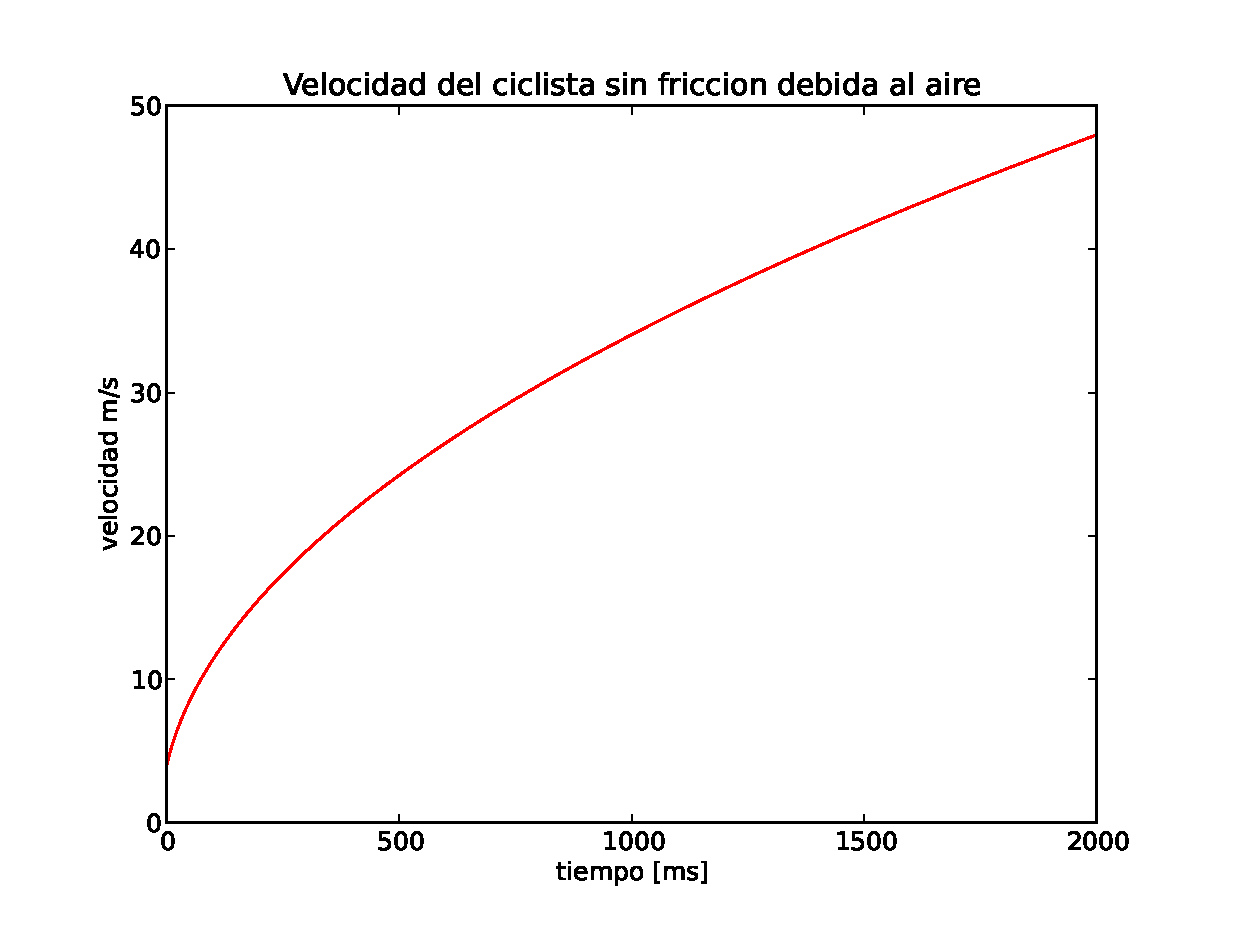
\includegraphics[scale=0.475]{Imagenes/EjerBicicleta01.eps}
\end{figure}
\end{frame}
\begin{frame}
\frametitle{Resultado ¿correcto?}
Consideremos que:
\setbeamercolor{item projected}{bg=amber,fg=black}
\setbeamertemplate{enumerate items}{%
\usebeamercolor[bg]{item projected}%
\raisebox{1.5pt}{\colorbox{bg}{\color{fg}\footnotesize\insertenumlabel}}%
}
\begin{enumerate}[<+->]
\item Hemos desarrollado un algoritmo que resuelve el problema inicial.
\item Los valores son consistentes.
\item La gráfica nos indica el comportamiento de la solución.
\end{enumerate}
\pause
Aún así: ¿debemos de considerar el problema como bien resuelto? \pause \textcolor{auburn}{No!}
\end{frame}

\section*{Considerando la fricción del aire}

\begin{frame}
\frametitle{Segunda aproximación}
La fuerza debida a la fricción puede aproximarse de manera inicial como:
\pause
\begin{equation}
F_{a} \simeq - B_{1} \, v - B_{2} v^{2}
\label{EqFfriccion}
\end{equation}
Para velocidades muy bajas, el primer término es el que domina, y el coeficiente $B_{1}$ se puede calcular para objetos con formas sencillas.
\end{frame}
\begin{frame}
\frametitle{El tamaño del  objeto}
Para una velocidad razonable $v^{2}$ el término domina sobre los demás, pero $B_{2}$ no puede calcularse exactamente en objetos sencillos como una pelota de beisbol, menos para una bicicleta.
\end{frame}
\begin{frame}
\frametitle{Haciendo otra aproximación}
Podemos aproximar el valor de $B_{2}$ como sigue:
\\
\bigskip
\pause
Si un objeto se mueve a través de la atmósfera, debe empujar fuera del camino el aire delante de él. 
\end{frame}
\begin{frame}
\frametitle{Haciendo otra aproximación}
La masa de aire movida en el tiempo $\dd{t}$ es $m_{\text{aire}} \sim \rho A \: v \: \dd{t}$, donde $\rho$ 
es la densidad del aire y $A$ el área frontal del objeto.
\\
\bigskip
\pause
Este aire tiene una velocidad de orden $v$, y por lo tanto, su energía cinética es $E_{\text{aire}} \sim m_{\text{aire}} \: v^{2} / 2$.
\end{frame}
\begin{frame}
\frametitle{Haciendo otra aproximación}
Este es también el trabajo realizado por la fuerza de arrastre (la fuerza sobre el objeto debido a la resistencia del aire) en el tiempo $\dd{t}$, por lo $F_{a} \: \dd{t} = E_{\text{aire}}$.
\\
\bigskip
\pause
Al juntar estos resultados, encontramos que:
\pause
\begin{align*}
F_{a} \simeq - C \: \rho \: A \: v^{2}
\end{align*}
\end{frame}
\begin{frame}
\frametitle{Nueva expresión}
Incluyendo este término en la expresión para la velocidad:
\pause
\begin{equation}
v_{i+1} = v_{i} + \dfrac{P}{m \: v_{i}} \Delta \: t - \dfrac{C \: \rho \: A \: v_{i}^{2}}{m} \: \Delta \: t
\label{Eqvelifriccion}
\end{equation}
\end{frame}
\begin{frame}
\frametitle{Pasando al código}
\textbf{Ejercicio a cuenta 2: } Implementar el código en \python, considerando los valores $C = 0.5$ y $A=0.33$.
\\
\bigskip
\pause
De tal manera que al obtener la gráfica de la solución, debes de presentar una figura con el siguiente resultado:
\end{frame}
\begin{frame}
\frametitle{Velocidad en las dos aproximaciones}
\begin{figure}[H]
	\centering
	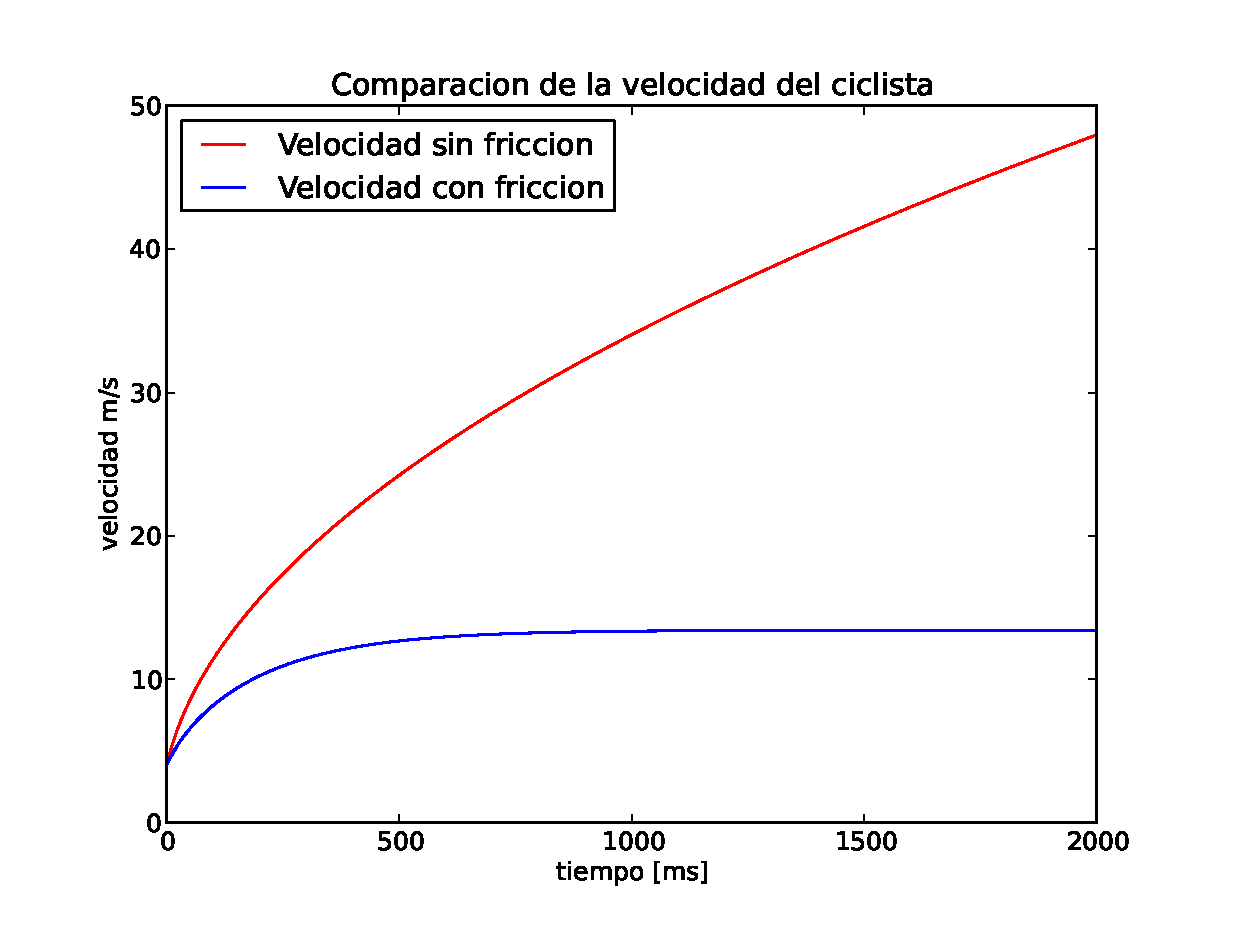
\includegraphics[scale=0.475]{Imagenes/EjerBicicleta02.eps}
\end{figure}
\end{frame}
\begin{frame}
\frametitle{Conclusión importante}
El resultado que tenemos a partir de nuestra solución numérica con la segunda aproximación, \textcolor{ao}{es más congruente con la física}.
\\
\bigskip
\pause
Nota que a pesar de tener un algoritmo que resuelve una ecuación de movimiento, nuestrto trabajo no termina con proporcionar una respuesta con el código, \pause sino que revisemos la consistencia de la solución con la física que ya manejamos.
\end{frame}
\begin{frame}
\frametitle{Ejercicio a cuenta:}
\textbf{Ejercicio a cuenta 3: } El número $ln 2$ se puede calcular de la serie:
\begin{align*}
\ln 2 = 1 - \dfrac{1}{2} + \dfrac{1}{3} -\dfrac{1}{4} + \ldots
\end{align*}
Se sabe del análisis que esta serie converge y que la magnitud del error en cualquier suma parcial es menor que la magnitud del primer término despreciado. Estima el número de términos que se requerirían para calcular $\ln 2$ con 10 decimales.
\end{frame}
\begin{frame}
\frametitle{Ejercicio a cuenta}
\textbf{Ejercicio a cuenta 4: } El 25 de febrero de 1991, durante la guerra del Golfo, una batería de misiles Patriot americanos en Dharan (Arabia Saudita) no lograron interceptar un misil Scud iraquí. Murieron 28 soldados americanos.
\end{frame}
\begin{frame}
\frametitle{Ejercicio a cuenta}
La causa: los errores numéricos por utilizar truncado en lugar de redondeo en el sistema que calcula el momento exacto en que debe ser lanzado el misil.
\\
\bigskip
\pause
Las computadoras de los Patriot que han de seguir la trayectoria del misil Scud, la predicen punto a punto en función de su velocidad conocida y del momento en que fue detectado por última vez en el radar.
\end{frame}
\begin{frame}
\frametitle{Ejercicio a cuenta}
La velocidad es un número real. El tiempo es una magnitud real pero el sistema la calculaba mediante un reloj interno que contaba décimas de segundo, por lo que representaban el tiempo como una variable entera.
\\
\bigskip
\pause
Cuanto más tiempo lleva el sistema funcionando más grande es el entero que representa el tiempo.
\end{frame}
\begin{frame}
\frametitle{Ejercicio a cuenta}
Las computadoras del Patriot almacenan los números reales representados en punto flotante con una mantisa de $24$ bits.
\\
\bigskip
\pause
Para convertir el tiempo entero en un número real se multiplica éste por $1/10$, y se trunca el resultado (en lugar de redondearlo). El número $1/10$ se almacenaba truncado a $24$ bits.
\end{frame}
\begin{frame}
\frametitle{Ejercicio a cuenta}
El pequeño error debido al truncado, se hace grande cuando se multiplica por un número (entero) grande, y puede conducir a un error significativo.
\\
\bigskip
La batería de los Patriot llevaba en funcionamiento más de $100$ horas, por lo que el tiempo entero era un número muy grande y el número real resultante tendrá un error cercano a $0.34$ segundos. \pause Explica a detalle qué fue lo que ocurrió.
\end{frame}
\begin{frame}
\frametitle{Lista de ejercicios del Tema 1}
Revisa en Moodle una lista de ejercicios del Tema 1, serán el tipo de ejercicios para el Examen-Tarea.
\end{frame}

% \begin{frame}
% \frametitle{Hablando de errores}
% El problema es que como científicos, queremos un resultado correcto o al menos en el que la incertidumbre sea pequeña y de tamaño conocido.
% \end{frame}
% \subsection{¿De dónde vienen los errores?}
% \begin{frame}
% \frametitle{Fuentes de errores computacionales}
% Existen al menos cuatro fuentes de errores que se pueden presentar en los cálculos computacionales:
% \pause
% \setbeamercolor{item projected}{bg=blue!70!black,fg=yellow}
% \setbeamertemplate{enumerate items}[circle]
% \begin{enumerate}[<+->]
% \item Un modelo equivocado.
% \item Errores aleatorios.
% \item Errores por aproximación
% \item Errores por redondeo.
% \end{enumerate}
% \end{frame}
% \subsection{Un modelo equivocado}
% \begin{frame}
% \frametitle{Un modelo equivocado}
% Se presentan cuando nuestra propuesta de modelo no es el pertinente, siendo quizá la parte más crítica ya que antes de continuar, debemos de repasar la parte de la física para resolver debidamente nuestro problema
% \end{frame}
% \begin{frame}
% \frametitle{Un modelo equivocado}
% También se consideran los errores tipográficos, introducir valores que no corresponden, ejecutar el programa incorrecto, usar el archivo de datos equivocado, etc.
% \\
% \bigskip
% Sugerencia: \pause \textoazul{Si el número de errores comienza a crecer, es momento de ir a casa o tomar un descanso.}
% \end{frame}
% \subsection{Errores aleatorios}
% \begin{frame}
% \frametitle{Errores aleatorios}
% Se presenta una imprecisión debida por acontecimientos tales como: fluctuaciones en la electrónica, incidencia de rayos cósmicos, o alguien que se tropieza con un enchufe.
% \\
% \bigskip
% Éstos errores pueden ser raros, pero no tenemos ningún control sobre ellos y su probabilidad aumenta conforme transcurre el tiempo.
% \end{frame}
% \subsection{Errores por aproximación}
% \begin{frame}
% \frametitle{Errores por aproximación}
% La imprecisión surge de la simplificación de las matemáticas para que un problema pueda ser resuelto en la computadora.
% \\
% \bigskip
% Incluyen la sustitución de series infinitas por sumas finitas, intervalos infinitesimales por finitos, y funciones variables por constantes.
% \end{frame}
% \begin{frame}
% \frametitle{Errores por aproximación}
% Por ejemplo
% \begin{align}
% \begin{aligned}
% \onslide<1->{\sin(x) &= \sum_{n = 1}^{\infty} \: \dfrac{(-1)^{n-1} \: x^{2n - 1}}{(2n - 1)!} \hspace{0.5cm} \mbox{(exacta)} \\[15pt]}
% \onslide<2->{& \simeq \sum_{n = 1}^{N} \: \dfrac{(-1)^{n-1} \: x^{2n - 1}}{(2n - 1)!} \hspace{0.5cm} \mbox{(algoritmo)} \pause \\[15pt]}
% \onslide<3>{& = \sin(x) + \varepsilon(x, N)}
% \end{aligned}
% \label{eq:ecuacion_02_02}
% \end{align}
% \pause
% donde $\varepsilon(x,N)$ es el error por la aproximación, en este caso $\varepsilon$ corresponde a los términos desde $N+1$ hasta $\infty$.
% \end{frame}
% \begin{frame}
% \frametitle{Errores por aproximación}
% Dado que el error por la aproximación se genera en el algoritmo que usamos para aproximar la matemática, también se le conoce como \underline{error del algoritmo}.
% \end{frame}
% \begin{frame}
% \frametitle{Errores por aproximación}
% Para una buena y razonable aproximación, el error debido por la aproximación debería de reducirse cuando el valor de $N$ se incrementa, y debería de anularse en el límite $N \rightarrow \infty$.
% \end{frame}
% \begin{frame}
% \frametitle{Errores por aproximación}
% Para el ejemplo (\ref{eq:ecuacion_02_02}), como la escala de $N$ se fija por el valor de $x$, un pequeño error de aproximación requiere que $ N \geqslant x$.
% \\
% \bigskip
% Por lo que si $x$ y $N$ son valores cercanos entre sí, el error de aproximación será grande.
% \end{frame}
% \subsection{Errores por redondeo}
% \begin{frame}
% \frametitle{Errores por redondeo}
% La imprecisión se genera por el número finito de dígitos utilizados para almacenar números de punto flotante.
% \\
% \bigskip
% Estos \enquote{errores} son análogos a la incertidumbre en la medición de una cantidad física encontrada en un laboratorio de física.
% \end{frame}
% \begin{frame}
% \frametitle{Errores por redondeo}
% El error general de redondeo se acumula a medida que el equipo maneja más números, es decir, a medida que aumenta el número de pasos en un cálculo, y puede hacer que algunos algoritmos se vuelvan inestables con un rápido aumento del error.
% \end{frame}
% \begin{frame}
% \frametitle{Errores por redondeo}
% En algunos casos, el error por redondeo puede convertirse en el componente principal en la respuesta, lo que lleva a lo que los expertos informáticos llaman \azulfuerte{basura}.
% \end{frame}
% \begin{frame}
% \frametitle{Errores por redondeo}
% Por ejemplo, si la computadora mantiene cuatro decimales, entonces almacenará $\frac{1}{3}$ como $0.3333$ y $\frac{2}{3} = 0.6667$, donde el equipo ha \enquote{redondeado} el último dígito en $\dfrac{2}{3}$.
% \end{frame}
% \begin{frame}
% \frametitle{Errores por redondeo}
% Por consiguiente, si hacemos en la computadora un cálculo tan simple como $2 \frac{1}{3} - \frac{2}{3}$, produce
% \begin{equation}
% 2 \left( \dfrac{1}{3} \right) - \dfrac{2}{3} = 0.6666 - 0.6667 = -0.0001 \neq 0
% \label{eq:ecuacion_02_03}
% \end{equation}
% \pause
% Aunque el resultado es pequeño, no es $0$, y si se repete este tipo millones de veces este cálculo, la respuesta final puede que ni siquiera sea pequeña (\textcolor{red}{la basura genera basura}).
% \end{frame}
% \section{Modelos para el desastre}
% \frame{\tableofcontents[currentsection, hideothersubsections]}
% \subsection{Definiciones}
% \begin{frame}[fragile]
% \frametitle{Definiciones}
% Sea $x^{*}$ el valor exacto de una cierta cantidad y $x$ la aproximación a esa cantidad.
% \\
% \bigskip
% Por definición, el valor absoluto asociado a $x$ es
% \begin{equation}
% \Delta = \vert x^{*} - x \vert 
% \label{eq:ecuacion_01_03}	
% \end{equation}
% \end{frame}
% \begin{frame}
% \frametitle{Definiciones}
% En general, los cálculos numéricos operan con aproximaciones tanto a las cantidades como a sus errores absolutos.
% \\
% \bigskip
% En el caso ideal, en el que, además de la aproximación $x$, también se conocería el error absoluto exacto, el número exacto sería exactamente expresable como
% \begin{equation}
% x^{*} = x \pm \Delta^{*}
% \label{eq:ecuacion_01_04}    	
% \end{equation}    
% \end{frame}
% \begin{frame}
% \frametitle{Definiciones}
% Sin embargo, en general, solo está disponible una estimación del error absoluto y, en consecuencia, solo un estimado del valor exacto puede determinarse:
% \begin{equation}
% x - \Delta \leq x^{*} \leq x + \Delta
% \label{eq:ecuacion_01_05}
% \end{equation}
% \end{frame}
% \begin{frame}
% \frametitle{Definiciones}
% Para que la estimación $x$ sea confiable, es importante que $\Delta$ no subestime el error verdadero, es decir, $\Delta \geq \Delta^{*}$, en este caso, se denomina \emph{limitación de error absoluto}.
% \end{frame}
% \begin{frame}
% \frametitle{Más definiciones}
% El error relativo $\delta^{*}$ es la aproximación de $x$ a $x^{*}$, y es igual al cociente del error absoluto con el número exacto:
% \begin{equation}
% \delta^{*} = \dfrac{\Delta^{*}}{\vert x^{*} \vert} \hspace{1cm} x^{*} \neq 0
% \label{eq:ecuacion_01_06}
% \end{equation}
% \end{frame}
% \begin{frame}
% \frametitle{Más definiciones}
% Re-emplazando $\Delta^{*}$ en la ecuación(\ref{eq:ecuacion_01_04}) de la ecuación (\ref{eq:ecuacion_01_06}), tendremos la expresión para un número exacto:
% \begin{equation}
% x^{*} \simeq x \: (1 \pm \delta^{*})
% \label{eq:ecuacion_01_07}
% \end{equation}
% \end{frame}
% \begin{frame}
% \frametitle{Más definiciones}
% Basándose en el error relativo de la aproximación $\delta \geq \delta^{*}$, se expresa el valor exacto como:
% \begin{equation}
% x^{*} \simeq x \: (1 \pm \delta)
% \label{eq:ecuacion_01_08}
% \end{equation}
% \end{frame}
% \section{Errores en las operaciones aritméticas}
% \frame{\tableofcontents[currentsection, hideothersubsections]}
% \subsection{Errores en las operaciones elementales}
% \begin{frame}
% \frametitle{Errores en las operaciones elementales}
% Revisaremos la forma en que varias operaciones elementales propagan los errores relativos de sus operandos.
% \\
% \bigskip
% En relación con los cálculos numéricos, las consideraciones desarrolladas a continuación se refieren específicamente a los errores de redondeo y truncamiento.
% \end{frame}
% \subsection{Error en la suma}
% \begin{frame}
% \frametitle{Error en la suma}
% Sea la suma de dos números próximos, $x_{1}$ y $x_{2}$, que tienen el mismo signo.
% \\
% \bigskip
% La suma evidentemente conserva el signo y acumula las magnitudes de los operandos:
% \begin{equation}
% x = x_{1} + x_{2}
% \label{eq:ecuacion_01_14}
% \end{equation}
% \end{frame}
% \begin{frame}
% \frametitle{Error en la suma}
% Tenemos que el error total es
% \[ \Delta x =  \Delta x_{1} + \Delta x_{2} \]
% \pause
% pero, dado que los errores individuales pueden, en función de sus signos, compensarse mutuamente y acumularse.
% \end{frame}
% \begin{frame}
% \frametitle{Error en la suma}
% La suma de los errores absolutos de los operandos proporciona en realidad un límite superior para el error absoluto total de la suma:
% \begin{equation}
% \Delta \leq \Delta_{1} + \Delta_{2}
% \label{eq:ecuacion_01_15}
% \end{equation}
% \end{frame}
% \begin{frame}
% \frametitle{Error relativo en la suma}
% El error relativo de la suma de dos números proximos del mismo signo no supera el error relativo más grande de los sumandos:
% \begin{equation}
% \delta \leq \max{(\delta_{1}, \delta_{2})}
% \label{eq:ecuacion_01_16}
% \end{equation}
% \end{frame}
% \subsection{Error en la diferencia}
% \begin{frame}
% \frametitle{Error en la diferencia}
% Ahora consideremos la diferencia de dos números próximos con \emph{el mismo signo}:
% \begin{equation}
% x = x_{1} - x_{2}
% \label{eq:ecuacion_01_18}
% \end{equation}
% \pause
% Debería ser evidente que las ecuaciones (\ref{eq:ecuacion_01_14}) y (\ref{eq:ecuacion_01_18}) cubren todas las posibles situaciones algebraicas.
% \end{frame}
% \begin{frame}
% \frametitle{Error en la diferencia}
% Al igual que en el caso de la suma, el caso más desfavorable es aquél en el que los errores absolutos se potencian entre sí, y, por lo tanto, la suma de los errores absolutos es, de nuevo, el límite superior para el error absoluto de la diferencia:
% \[ \Delta \leq  \Delta_{1} + \Delta_{2} \]
% \end{frame}
% \begin{frame}
% \frametitle{Error en la diferencia}
% Maximizando el error absoluto total en la definición de error relativo ($\delta$), tenemos que
% \begin{equation}
% \delta \leq \dfrac{\Delta_{1} + \Delta_{2}}{\vert x_{1} - x_{2} \vert} = \dfrac{\vert x_{1} \vert \: \delta_{1} + \vert x_{2} \vert \: \delta_{2}}{\vert x_{1} - x_{2} \vert}
% \end{equation}
% \end{frame}
% \begin{frame}
% \frametitle{Error en la diferencia}
% Si los sumandos están cerca de su valor, la diferencia absoluta $\vert x_{1} - x_{2} \vert$ es pequeño e, incluso para pequeños errores relativos individuales, $\delta_{1}$ y $\delta_{2}$, el error relativo de la diferencia, $\delta$, puede volverse significativo.
% \end{frame}
% \subsection{Error en el producto}
% \begin{frame}
% \frametitle{Error en el producto}
% El error relativo de un producto de dos números próximos $x = x_{1} \: x_{2}$, no excede a la suma del error relativo de los factores $\delta_{1}$ y $\delta_{2}$:
% \begin{equation}
% \delta = \delta_{1} + \delta_{2}
% \label{eq:ecuacion_01_20}
% \end{equation}
% \end{frame}
% \subsection{Error en el cociente}
% \begin{frame}
% \frametitle{Error en el cociente}
% Consideremos ahora el cociente
% \[ x = \dfrac{x_{1}}{x_{2}} \]
% de dos números próximos no nulos.
% \\
% \bigskip
% \pause
% Teniendo en cuenta, una vez más, que $x_{1}$ y $x_{2}$ se ven afectados por pequeños errores absolutos $\Delta_{1} = \vert \Delta x_{1} \vert$ y $\Delta_{2} = \vert \Delta x_{2} \vert$:
% \end{frame}
% \begin{frame}
% \frametitle{Error en el cociente}
% Obtenemos la relación límite:
% \begin{equation}
% \delta = \delta_{1} + \delta_{2}
% \label{eq:ecuacion_01_27}
% \end{equation}
% que establece que el error relativo del cociente no excede los errores relativos acumulados del dividendo y divisor.
% \end{frame}
% \section{Errores en las funciones esféricas de Bessel}
% \frame[allowframebreaks]{\tableofcontents[currentsection, hideothersubsections]}
% \subsection{Funciones de Bessel}
% \begin{frame}
% \frametitle{Funciones de Bessel}
% La acumulación de errores por redondeo a menudo limita la capacidad de un programa para calcular con precisión.
% \\
% \bigskip
% \pause
% Revisaremos como ejercicio, la manera de calcular las funciones esféricas de Bessel $j_{\ell}(x)$ y de Neumann $n_{\ell}(x)$.
% \end{frame}
% \begin{frame}
% \frametitle{Funciones de Bessel}
% Estas funciones son respectivamente, las soluciones regulares/irregulares (no singulares / singulares en el origen) de la ecuación diferencial
% \begin{equation}
% x^{2} \: f^{\prime \prime} (x) + 2 \: x \: f^{\prime}(x) + [ x^{2} - \ell ( \ell + 1)] \: f(x) = 0
% \label{eq:ecuacion_02_19}
% \end{equation}
% \end{frame}
% \begin{frame}
% \frametitle{Funciones de Bessel y esféricas de Bessel}
% Las funciones esféricas de Bessel se relacionan con las funciones de Bessel de primera clase por
% \[ j_{\ell}(x) = \sqrt{\dfrac{\pi}{2 \: x}} \: J_{n + \frac{1}{2}} (x) \]
% \end{frame}
% \begin{frame}
% \frametitle{Funciones de Bessel y esféricas de Bessel}
% Se encuentran en diversos problemas de la física, como la expansión de una onda plana en ondas esféricas parciales
% \begin{equation}
% e^{i \: \mathbf{k \cdot r}} = \sum_{\ell = 0}^{\infty} i^{\ell} \: (2 \: \ell + 1) \: j_{\ell} (k \:  r) \: P_{\ell}(\cos \theta)
% \label{eq:ecuacion_02_20}
% \end{equation}    
% \end{frame}
% \begin{frame}
% \frametitle{Funciones esféricas de Bessel de orden $n$}
% \fontsize{12}{12}\selectfont
% A continuación se muestra una gráfica con las funciones esféricas de Bessel de orden $n = 0, \ldots, 5$:
% \begin{figure}
% \centering
% 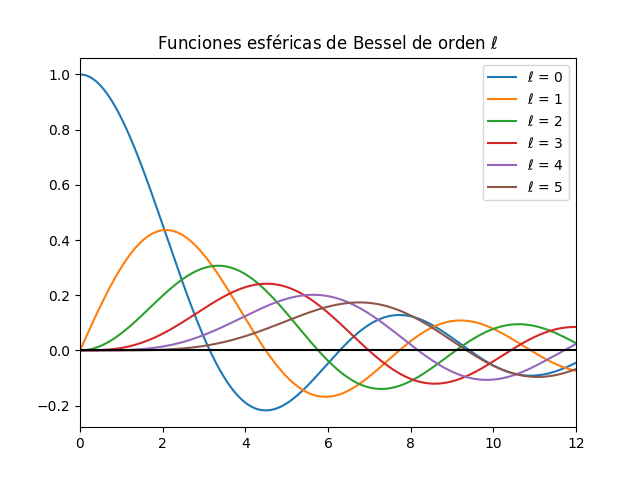
\includegraphics[scale=0.4]{funcionesEsfericasBessel}
% \caption{La gráfica se generó usando la librería de funciones especiales de \python.}
% %\caption{Nótese que para valores pequeños de $x$, los valores para un $\ell$ mayor, se hacen prograsivamente más pequeños.}
% \end{figure}
% \end{frame}
% \begin{frame}
% \frametitle{Valores para $\ell = 0, 1$}
% Los dos primero valores para $\ell$ son
% \begin{align}
% j_{0} (x) &= + \dfrac{\sin x}{x}, \hspace{1cm} j_{1} (x) = +\dfrac{\sin x}{x^{2}} - \dfrac{\cos x}{x} \label{eq:ecuacion_02_21} \\
% &{} \nonumber \\
% n_{0} (x) &= - \dfrac{\cos x}{x}, \hspace{1cm} n_{1} (x) = -\dfrac{\cos x}{x^{2}} - \dfrac{\sin x}{x} \label{eq:ecuacion_02_22}
% \end{align}
% \end{frame}
% \subsection{Ejercicio: Relaciones de recursión}
% \begin{frame}
% \frametitle{Relaciones de recursión}
% La manera clásica de calcular las funciones de Bessel de orden $j$: $j_{\ell} (x)$ es sumar su serie de potencias para valores pequeños de $\frac{x}{\ell}$ y sumando su expansión asintótica para valores de $x$ grandes.
% \end{frame}
% \begin{frame}
% \frametitle{Relaciones de recurrencia}
% El enfoque que usaremos, se basa en \emph{las relaciones de recurrencia}:
% \begin{align}
% j_{\ell + 1} (x) = \dfrac{2 \: \ell + 1}{x} \: j_{\ell}(x) - j_{\ell - 1}(x) \hspace{0.5cm} \mbox{hacia arriba} \label{eq:ecuacion_02_23}  \\
% {} \nonumber \\ 
% j_{\ell - 1} (x) = \dfrac{2 \: \ell + 1}{x} \: j_{\ell}(x) - j_{\ell + 1}(x) \hspace{0.5cm} \mbox{hacia abajo} \label{eq:ecuacion_02_24}
% \end{align}
% \end{frame}
% \begin{frame}
% \frametitle{Relaciones de recurrencia}
% Las ecuaciones (\ref{eq:ecuacion_02_23}) y (\ref{eq:ecuacion_02_24}) son la misma relación:
% \setbeamercolor{item projected}{bg=blue!70!black,fg=yellow}
% \setbeamertemplate{enumerate items}[circle]
% \begin{enumerate}[<+->]
% \item Una escrita para la recurrencia hacia adelante que parte de valores pequeños a valores grandes de $\ell$.
% \item La otra relación de recurrencia es descendente para valores de $\ell$ pequeños.
% \end{enumerate}
% \pause
%  Con unas cuantas sumas y multiplicaciones, las relaciones de recurrencia permiten el cálculo rápido y sencillo de todo el conjunto de valores de $j_{\ell}$ para $x$ fijo y todo $\ell$.
% \end{frame}
% \begin{frame}
% \frametitle{Relaciones de recurrencia}
% Para la relación de recurrencia hacia adelante de $\ell$ para un $x$ fijo, comenzamos con las formas conocidas para $j_{0}$ y $j_{1}$ (\ref{eq:ecuacion_02_21}) y usamos (\ref{eq:ecuacion_02_23}).
% \end{frame}
% \begin{frame}
% \frametitle{Relaciones de recurrencia}
% Como veremos, esta recurrencia hacia adelante parece funcionar al principio, pero luego falla.
% \\
% \bigskip
% La razón de la falla se puede ver en las gráficas de $j_{\ell}(x)$ y $n_{\ell}(x)$ como función de $x$.
% \end{frame}
% \begin{frame}
% \frametitle{Relaciones de recurrencia}
% \begin{figure}
% \centering
% 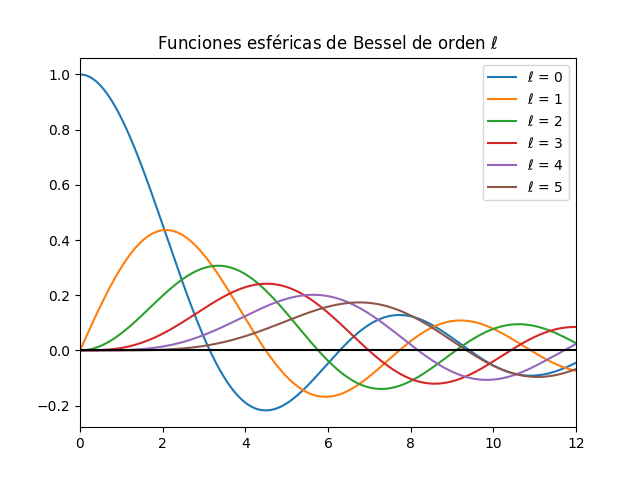
\includegraphics[scale=0.5]{funcionesEsfericasBessel}
% \end{figure}
% \end{frame}
% \begin{frame}
% \frametitle{Relaciones de recurrencia}
%  Si iniciamos con  $x \simeq 2$ y $\ell = 0$, veremos que a medida que la  recurrencia hacia adelante para  $j_{\ell}$ con valores mayores de $\ell$ con (\ref{eq:ecuacion_02_23}), esencialmente tomamos la diferencia de dos funciones \enquote{grandes} para producir un valor \enquote{pequeño} para $j_{\ell}$.
% \end{frame}
% \begin{frame}
% \frametitle{Relaciones de recurrencia}
% Este proceso sufre de cancelación sustractiva y siempre reduce la precisión.
% \\
% \bigskip
% A medida que continuamos con la recurrencia, tomamos la diferencia de dos funciones pequeñas con errores grandes y producimos una función más pequeña con un error aún mayor. Después de cierto tiempo, nos quedamos con sólo el error de redondeo (basura).
% \end{frame}
% \begin{frame}
% \frametitle{Estimando el error}
% Para ser más específicos, llamemos $j_{\ell}^{(c)}$ al valor numérico que calculamos como nua aproximación para $j_{\ell}(x)$.
% \\
% \bigskip
% Por lo que si comenzamos con un valor neto $j_{\ell}$, después de un corto tiempo la falta de precisión de la computadora se mezcla efectivamente en un poco de $n_{\ell}$:
% \begin{equation}
% j_{\ell}^{(c)} = j_{\ell} (x) + \varepsilon \: n_{\ell} (x)
% \label{eq:ecuacion_02_25}	
% \end{equation}
% \end{frame}
% \begin{frame}
% \frametitle{Estimando el error}
% Esto no lo podemos evitar, porque tanto $j_{\ell}$ como $n_{\ell}$ satisfacen la misma ecuación diferencial y, por esa razón, la misma relación de recurrencia.
% \\
% \bigskip
% La mezcla de $n_{\ell}$ se convierte en un problema cuando el valor numérico de $n_{\ell}(x)$ es mucho mayor que el de $j_{\ell} (x)$ porque incluso una cantidad minúscula de un número muy grande puede ser grande.
% \end{frame}
% \begin{frame}
% \frametitle{Estimando el error}
% Por el contrario, si usamos la relación de recurrencia hacia adelante (\ref{eq:ecuacion_02_23}) para generar la función esférica de Neumann $n_{\ell}$, no habrá ningún problema porque estamos combinando funciones pequeñas para producir más grandes, ya que es un proceso que no contiene cancelación sustractiva.
% \end{frame}
% \begin{frame}
% \frametitle{Solución al problema}
% La solución simple a este problema es usar (\ref{eq:ecuacion_02_24}) para la recursión descendente de los valores de $j_{\ell}$ que comienzan en un valor grande $\ell = L$.
% \\
% \bigskip
% Esto evita la cancelación sustractiva tomando valores pequeños de $j_{\ell + 1} (x)$ y $j_{\ell}(x)$ y generando por la suma un valor mayor en $j_{\ell -1}(x)$.
% \end{frame}
% \begin{frame}
% \frametitle{Solución al problema}
% Mientras que el error todavía puede mantenerse como una función de Neumann, la magnitud real del error disminuirá rápidamente conforme la recurrencia hacia atrás use valores pequeños de $\ell$.
% \end{frame}
% \begin{frame}
% \frametitle{Solución al problema}
% De hecho, si empezamos iterando hacia atrás con valores arbitrarios para $j_{L + 1}^{(x)}$ y $j_{L}^{(c)}$, después de un corto tiempo llegaremos a la correcta relación de $\ell$ para este valor de $x$.
% \end{frame}
% \begin{frame}
% \frametitle{Solución al problema}
% Aunque el valor numérico de $j_{0}^{c}$ así obtenido no será correcto porque depende de los valores arbitrarios asumidos para $j_{L + 1}$ y $j_{L}^{(c)}$, los valores relativos serán precisos. 
% \end{frame}
% \begin{frame}
% \frametitle{Solución al problema}
% Los valores absolutos se fijan a partir del valor conocido (\ref{eq:ecuacion_02_21}), $j_{0} (x) = \sin x / x$.
% \\
% \bigskip
% Debido a que la relación de recurrencia es una relación lineal entre los valores de $j_{\ell}$, sólo necesitamos normalizar todos los valores calculados mediante 
% \end{frame}
% \begin{frame}
% \frametitle{Solución al problema}
% \begin{equation}
% j_{\ell}^{\text{normalizada}} = j_{\ell}^{(c)} (x) \times \dfrac{j_{0}^{\text{analitica}}}{j_{0}^{(c)}}
% \label{eq:ecuacion_02_26}
% \end{equation}
% En consecuencia, después de haber terminado la recurrencia hacia abajo, se obtendrá la respuesta final normalizando todos los valores de $j_{\ell}^{(c)}$ basados en el valor conocido para $j_{0}$.
% \end{frame}
% \begin{frame}[fragile]
% \frametitle{Propuesta de código}
% Veamos la manera de implementar un código con \python para calcular el valor de la función esférica de Bessel con la recurrencia hacia atrás.
% \end{frame}
% \begin{frame}[allowframebreaks, fragile]
% \frametitle{Propuesta de código}
% \begin{lstlisting}[caption=Usando la regla de recurrencia hacia atrás, style= FormattedNumber, basicstyle=\linespread{0.9}\ttfamily\small, columns=fullflexible]
% import numpy as np
% import matplotlib.pyplot as plt
% import scipy.special as spl

% Xmax = 40.
% Xmin = 0.25
% paso = 0.1
% orden = 10
% inicio = 50

% def abajo (x, n, m):
%      j = np.zeros( (inicio + 2), float)
%      j[m+_1_] = j[m] = 1.
     
%      for k in range(m, 0, -1):
%          j[k-_1_] = ((2.*k + 1.)/x)*j[k] - j[k+_1_]
     
%      escala = (np.sin(x)/x)/j[0]
     
%      return j[n] * escala

% valoresy = []

% valoresx = []

% for x in np.arange(Xmin, Xmax, paso):
%     valoresy.append(abajo(x, orden, inicio))
%     valoresx.append(x)

% plt.plot(valores_x, valores_y, color='r')
% plt.axhline(y=0, ls='dashed', color = 'k')
% plt.xlim([0.25, 40])
% plt.show()
% \end{lstlisting}
% \end{frame}
% \begin{frame}
% \frametitle{Función aproximada}
% \begin{figure}
% \centering
% 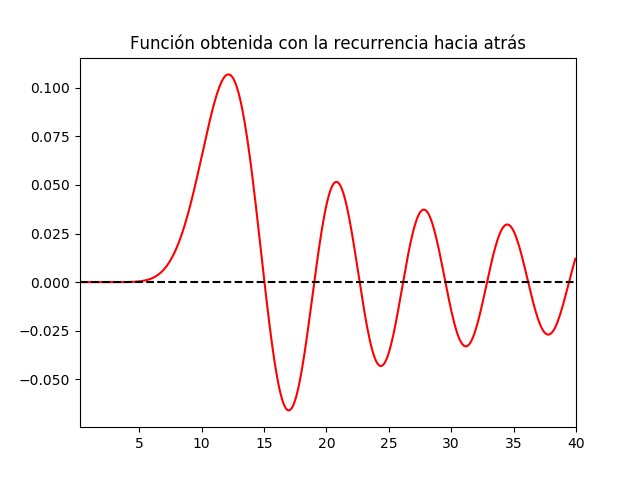
\includegraphics[scale=0.5]{funcionesEsfericasBessel_02}
% \caption{Gráfica obtenida con el algoritmo propuesto}
% \end{figure}
% \end{frame}



\end{document}